\documentclass{article}
\usepackage{graphicx}
\usepackage{titletoc}
\usepackage{titlesec}
\usepackage{geometry} 
\usepackage{fontspec, xunicode, xltxtra}
\usepackage{float}
\usepackage{cite}
\usepackage{amsmath}
\usepackage{listings}
\usepackage{titletoc}

\geometry{left=3cm,right=3cm,top=3cm,bottom=3cm}
\DeclareMathOperator*{\argmin}{argmin}
\DeclareMathOperator*{\argmax}{argmax}
\DeclareMathOperator*{\var}{var}
\DeclareMathOperator*{\expec}{E}

\begin{document}
\title{\textsf{Homework 1 for Bayesian Data Analysis}}
\author{Fan JIN\quad (2015011506)}
\maketitle

\section*{Question 2.1}
{
    The likelihood goes like $$p{(y\le 3 | \theta)} = \sum_{j=0}^{3} {\binom{n}{j} \theta^{j} (1-\theta)^{n-j}}$$

    Thus, the posterior distribution is $$p{(\theta | y\le 3)} \propto p{(\theta)} p{(y\le 3 | \theta)} \propto \sum_{j=0}^{3} {\binom{n}{j} \theta^{j+3} (1-\theta)^{n-j+3}}$$, where $n=10$. Here is its sketch.

    \begin{figure}[H]
        \centering
        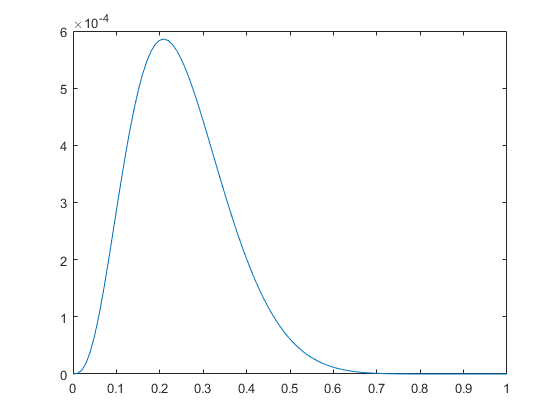
\includegraphics[width = 0.7\linewidth]{1.png}
        \caption{Posterior density of $\theta$}
    \end{figure}
}

\section*{Question 2.2}
{
    Denote $A$ as the event that the first two spins are tail. We have the likelihood $$p{(A | C_1)} = 0.16$$ and $$p{(A | C_2)} = 0.36$$

    So, the posterior probabilities are $$p{(C_1 | A)} \propto p{(C_1)} p{(A | C_1)} = 0.08$$ and $$p{(C_2 | A)} \propto p{(C_2)} p{(A | C_2)} = 0.18$$ 

    Denote $y$ as the number of additional spins until a head shows up. We have $$E{(y | A)} = \frac{p{(C_1 | A)} E{(y | A, C_1)} + p{(C_2 | A)} E{(y | A, C_2)}}{p{(C_1 | A)} + p{(C_2 | A)}} $$ $$= \frac{p{(C_1 | A)} E{(y | C_1)} + p{(C_2 | A)} E{(y | C_2)}}{p{(C_1 | A)} + p{(C_2 | A)}} $$ $$= \frac{0.08 * (1/0.6) + 0.18 * (1/0.4)}{0.08 + 0.18} = 2.2436$$
}

\section*{Question 2.3b}
{
    $$y \sim \mathrm{Bin}(n, p),$$ where $n=1000$ and $p=1/6$. Since $n=1000$ is large and $p=1/6$ is not close to $0$ or $1$, we can apply the normal approximation of binomial distribution here: $$y \sim \mathrm{Norm}(np, np(1-p))$$

    Using the normal distribution table, we have the quantiles as follows.

    \begin{table}[!hbp]
        \begin{tabular}{|c|c|}
        \hline
        Quantile & Point \\
        \hline
        0.05 & 147.2819 \\
        \hline
        0.25 & 158.7177 \\
        \hline
        0.50 & 166.6667 \\
        \hline
        0.75 & 174.6156 \\
        \hline
        0.95 & 186.0515 \\
        \hline
        \end{tabular}
    \end{table}
}

\section*{Question 2.5a}
{
    $$\Pr{(y=k)} = \int_0^1 {\Pr{(y=k | \theta)}\mathrm{d}\theta}$$
    $$= \int_0^1 {\binom{n}{k} \theta^{k} (1-\theta)^{n-k}\mathrm{d}\theta}$$
    $$= \binom{n}{k} \int_0^1 {\theta^{k} (1-\theta)^{n-k}\mathrm{d}\theta}$$
    $$= \binom{n}{k} \mathrm{Beta}(k+1, n-k+1) = \frac{1}{n+1}$$
}

\section*{Question 2.5b}
{
    $$p(\theta | y) \propto \Pr{(y | \theta)} \Pr{(\theta)} \propto \theta^{y} (1-\theta)^{n-y} \theta^{\alpha-1} (1-\theta)^{\beta-1}$$
    $$\propto \theta^{y+\alpha-1} (1-\theta)^{n-y+\beta-1}$$
    Therefore, the posterior distribution of $\theta$ is $\mathrm{Beta}(y+\alpha, n-y+\beta)$, with its mean
    $$E(\theta | y) = \frac{y+\alpha}{n+\alpha+\beta}$$
    Since
    $$\frac{y+\alpha}{n+\alpha+\beta} - \frac{\alpha}{\alpha+\beta} = \frac{\beta y - \alpha (n-y)}{(n+\alpha+\beta)(\alpha+\beta)}$$
    and
    $$\frac{y+\alpha}{n+\alpha+\beta} - \frac{y}{n} = \frac{-\beta y + \alpha (n-y)}{(n+\alpha+\beta)n}$$
    have opposite sign, the posterior mean of $\theta$ must be between $\frac{\alpha}{\alpha+\beta}$ and $\frac{y}{n}$.
    
}

\section*{Question 2.5c}
{
    The prior variance is $1/12$, and the posterior variance is $\frac{(y+1)(n-y+1)}{(n+2)^2 (n+3)}$ (by the property of Beta distribution). 
    $$\frac{(y+1)(n-y+1)}{(n+2)^2 (n+3)} - \frac{1}{12}$$
    $$= \frac{12 (y+1)(n-y+1) - (n+2)^2 (n+3)}{12 (n+2)^2 (n+3)}$$
    $$\le \frac{12 (n/2+1)(n-n/2+1) - (n+2)^2 (n+3)}{12 (n+2)^2 (n+3)}$$
    $$= \frac{-n}{12(n+3)} \le 0$$
}

\section*{Question 2.5d}
{
    Note that the variance of $\mathrm{Beta}(\alpha, \beta)$ distribution is $$\frac{\alpha \beta}{(\alpha+\beta)^2 (\alpha+\beta+1)}$$ Try many parameters in R, and we find that the variance increases after observation for $\alpha=1$, $\beta=5$, $n=2$, and $y=1$.
}

\section*{Question 2.8a}
{
    $$p(\theta | \bar{y}=150) \propto \exp{((\frac{\theta-180}{40})^2)} \cdot \exp{((\frac{150-\theta}{20/\sqrt{n}})^2)}$$
    $$= \exp{((\frac{\theta-180}{40})^2 + (\frac{150-\theta}{20/\sqrt{n}})^2)}$$
    $$\propto \exp{((\frac{\theta-\mu}{\sigma})^2)},$$
    which is normalized to a normal distribution with mean $\mu$ and variance $\sigma^2$, where 
    $$\frac{1}{\sigma^2} = \frac{1}{40^2} + n \frac{1}{20^2},$$
    $$\mu = \sigma^2 (\frac{180}{40^2} + n \frac{150}{20^2}).$$
}

\section*{Question 2.8b}
{
    The posterior predictive distribution of $\widetilde{y}$ is a normal distribution with mean $\mu$ and variance $\sigma^2 + 20^2$, where $\mu$ and $\sigma^2$ is defined in Question 2.8a.
}

\section*{Question 2.8c}
{
    For $n=10$, calculate $\mu = 150.7317$ and $\sigma^2 = 39.02439$. the posterior predictive distribution of $\widetilde{y}$ is $\mathrm{Normal}(150.7317, 439.02439)$.
}

\section*{Question 2.8d}
{
    For $n=100$, calculate $\mu = 150.0748$ and $\sigma^2 = 3.990025$. the posterior predictive distribution of $\widetilde{y}$ is $\mathrm{Normal}(150.0748, 403.990025)$.
}

\section*{Question 2.19a}
{
    Assume the likelihood is proportional to $\theta \exp{(-\theta y)}$, and prior distribution of $\theta$ is $\mathrm{Gamma}(\alpha, \beta)$, that is
    $$p(\theta) \propto \theta^{\alpha-1} \exp{(-\beta \theta)}$$
    So, the posterior distribution is
    $$p(\theta | y) \propto \theta^{\alpha} \exp{(-(\beta + y) \theta)},$$
    which follows a $\mathrm{Gamma}(\alpha+1, \beta+y)$. Thus, the gamma distribution is the conjugate distribution for the exponential likelihood.
}

\section*{Question 2.19b}
{
    $$p(\theta) \propto \theta^{\alpha-1} \exp{(-\beta \theta)}$$
    By chain rule, one has
    $$p(\phi) \propto (\frac{1}{\phi^2}) \cdot (\frac{1}{\phi})^{\alpha-1} \exp{(-\beta (\frac{1}{\phi}))} = \phi^{-\alpha-1} \exp{(-\frac{\beta}{\phi})}$$
    This is an inverse-gamma distribution.
}

\section*{Question 2.19c}
{
    From Question 2.19a, after $n$ experiments, $$\theta|y_1,\cdots,y_n \sim \mathrm{Gamma}(\alpha+n, \beta+t(n))$$
    For the $\mathrm{Gamma}(\alpha, \beta)$ distribution, the coefficient of variation is $1/\sqrt{\alpha}$. So, we have
    $$\frac{1}{\sqrt{\alpha}} = 0.5$$ and $$\frac{1}{\sqrt{\alpha+n}} = 0.1$$
    That goes to $\alpha = 4$ and $n=96$.
}

\section*{Question 2.19d}
{
    The likelihood of $y$ about $\phi$, after $n$ experiments, is $$\frac{1}{\phi^n} \exp{(-\frac{y_1 + \cdots + y_n}{\phi})}$$
    Thus, the posterior distribution is $$\frac{1}{\phi^n} \exp{(-\frac{y_1 + \cdots + y_n}{\phi})} \cdot \phi^{-\alpha-1} \exp{(-\frac{\beta}{\phi})}$$
    $$= \phi^{-(\alpha+n)-1} \exp{(-\frac{\beta + y_1 + \cdots + y_n}{\phi})},$$
    which is an Inverse-gamma$(\alpha+n, \beta+t(n))$ distribution.

    For the Inverse-gamma$(\alpha, \beta)$ distribution, the coefficient of variation is $1/\sqrt{\alpha-2}$. So, we have
    $$\frac{1}{\sqrt{\alpha-2}} = 0.5$$ and $$\frac{1}{\sqrt{\alpha+n-2}} = 0.1$$
    That goes to $\alpha = 6$ and $n=96$.

    The answer does not change, despite that they have different $\alpha$s.
}

\section*{Question 2.20a}
{
    $$p(y\geq 100 | \theta) = \int_{100}^{+\infty} {\theta \exp{(-\theta y)} \mathrm{d}y} = \exp{(-100\theta)}$$
    $$p(\theta | y\geq 100) \propto \theta^{\alpha-1} \exp{(-\beta \theta)} \cdot \exp{(-100\theta)} = \theta^{\alpha-1} \exp{(-(\beta+100)\theta)}$$
    The posterior distribution $$\theta | y\geq 100 \sim \mathrm{Gamma}(\alpha, \beta+100),$$ with mean $\frac{\alpha}{\beta+100}$ and variance $\frac{\alpha}{(\beta+100)^2}$.
}

\section*{Question 2.20b}
{
    $$p(y=100 | \theta) = \theta \exp{(-100\theta)}$$
    $$p(\theta | y\geq 100) \propto \theta^{\alpha-1} \exp{(-\beta \theta)} \cdot \theta\exp{(-100\theta)} = \theta^{\alpha+1-1} \exp{(-(\beta+100)\theta)}$$
    The posterior distribution $$\theta | y\geq 100 \sim \mathrm{Gamma}(\alpha+1, \beta+100),$$ with mean $\frac{\alpha+1}{\beta+100}$ and variance $\frac{\alpha+1}{(\beta+100)^2}$.
}

\section*{Question 2.20c}
{
    In formula 2.8, we have $$\var{(\theta)} = \expec{(\var{(\theta|y)})} + \var{(\expec{(\theta|y)})} \geq \expec{(\var{(\theta|y)})}.$$
    
    The means the prior variance is, \emph{on average}, greater than the posterior variance. The second term here $\expec{(\var{(\theta|y)})}$ is the expectation of posterior variance with respect to $y$, which is different from the posterior variance itself:
    $$\expec{(\var{(\theta|y)})} \neq \var{(\theta|y)}$$

    In this case, however, we focus on specific $y$s ($y=100$ and $y\geq 100$). Therefore, the formula 2.8 does not apply here since it holds for the expectation of all possible $y$s.
}

\clearpage
\end{document}
